% Cover letter using letter.cls
\documentclass[a4paper]{scrreprt} 
%\usepackage{helvetica} % uses helvetica postscript font (download helvetica.sty)
%\usepackage{newcent}   % uses new century schoolbook postscript font 
\usepackage[utf8]{inputenc}
\usepackage{graphicx}
\usepackage{amsmath}
\usepackage{eurosym}
\usepackage{cite}
\usepackage{tabularx}
\usepackage{bytefield}
\usepackage{color}
\usepackage{longtable}
\usepackage{tabularx}
% the following commands control the margins:
%\topmargin=-1in    % Make letterhead start about 1 inch from top of page 
%\textheight=8.5in    % text height can be bigger for a longer letter
%\oddsidemargin=0pt   % leftmargin is 1 inch
%\textwidth=6.5in     % textwidth of 6.5in leaves 1 inch for right margin
\title{Implementing a temperature and humidity sensor network for the nEDM
experiment setup}
\author{Wenwen Chen, Rainer Schönberger}
\begin{document}
\maketitle
\tableofcontents
\input{Concept}
\section{Features}
\section{Sensors}
\subsection{TSIC 506F}
For temperature measurements, we use the TSIC 506F temperature sensor
integrated circuit. At a relatively low price of about \EUR{7} per device, it
is able to deliver very high accuracy (see table \ref{tab:tsic}).\\
The temperature is converted to a digital value, which is sent out over a
proprietary one wire protocol variant, called \emph{ZAC-Wire} (details see section \ref{chap:zac}).\\
In order to minimize soldering heat, which would influence the calibration, we used the TO92 packaged sensor.
\begin{table}[Hh!]
	\centering
	\begin{tabular}{| r | c |}
		\hline
		Temperature range & $-10\,^{\circ}\mathrm{C}$ to $-10\,^{\circ}\mathrm{C}$\\
		\hline
		Calibrated accuracy & $\pm 0.1\,\mathrm{K}$  \\
		\hline
		Resolution & $0.034\,\mathrm{K}$  \\
		\hline
	\end{tabular}
	\caption{TSIC 506F specs}
	\label{tab:tsic}
\end{table}
\subsection{HYT271}
\section{Logical design}
\begin{figure}
	\centering
	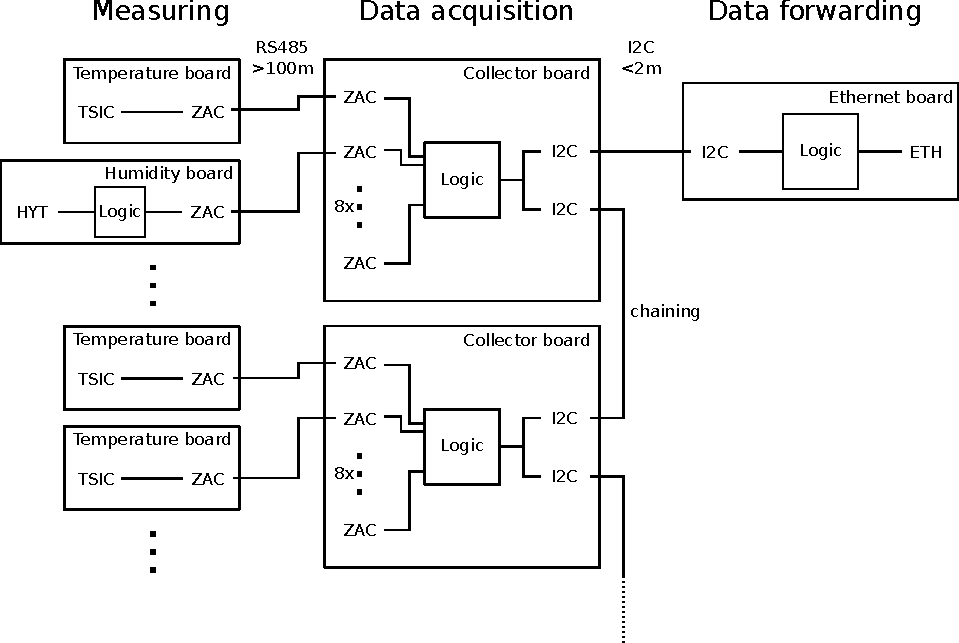
\includegraphics[width=0.9\textwidth]{img/plan2.pdf}
	\caption{Network topology}
	\label{fig:topo}
\end{figure}
\section{Protocols}
\subsection{ZAC}\label{chap:zac}
\begin{figure}
	\centering
	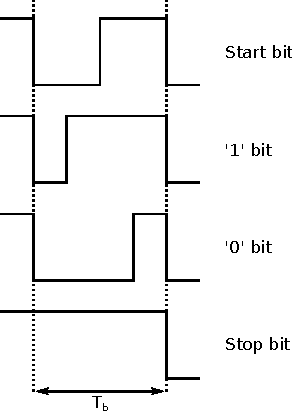
\includegraphics[width=0.3\textwidth]{img/zac_bits.pdf}
	\caption{ZAC protocol signal interpretation}
	\label{fig:zac}
\end{figure}
\begin{figure}
	\centering
	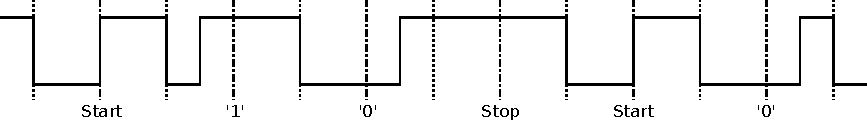
\includegraphics[width=0.9\textwidth]{img/zac_example.pdf}
	\caption{ZAC protocol example}
	\label{fig:zacexample}
\end{figure}
\subsection{I2C}
\subsection{RS485}
\input{Implementation}
\section{Temperature board}
\begin{figure}
	\centering
	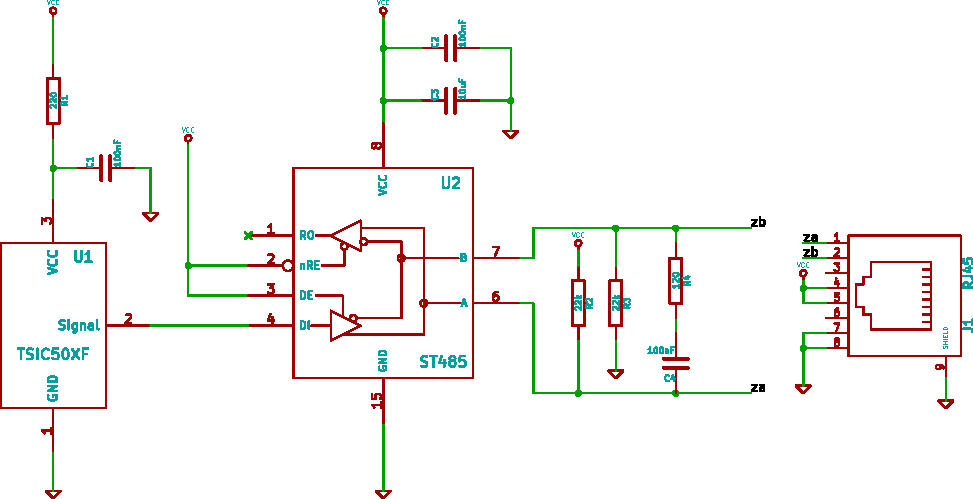
\includegraphics[width=0.6\textwidth]{img/schem_temperature_board.pdf}
	\caption{Temperature board schematic}
	\label{fig:schem_temp}
\end{figure}
\section{Humidity board}
\subsection{Hardware}
\begin{figure}
	\centering
	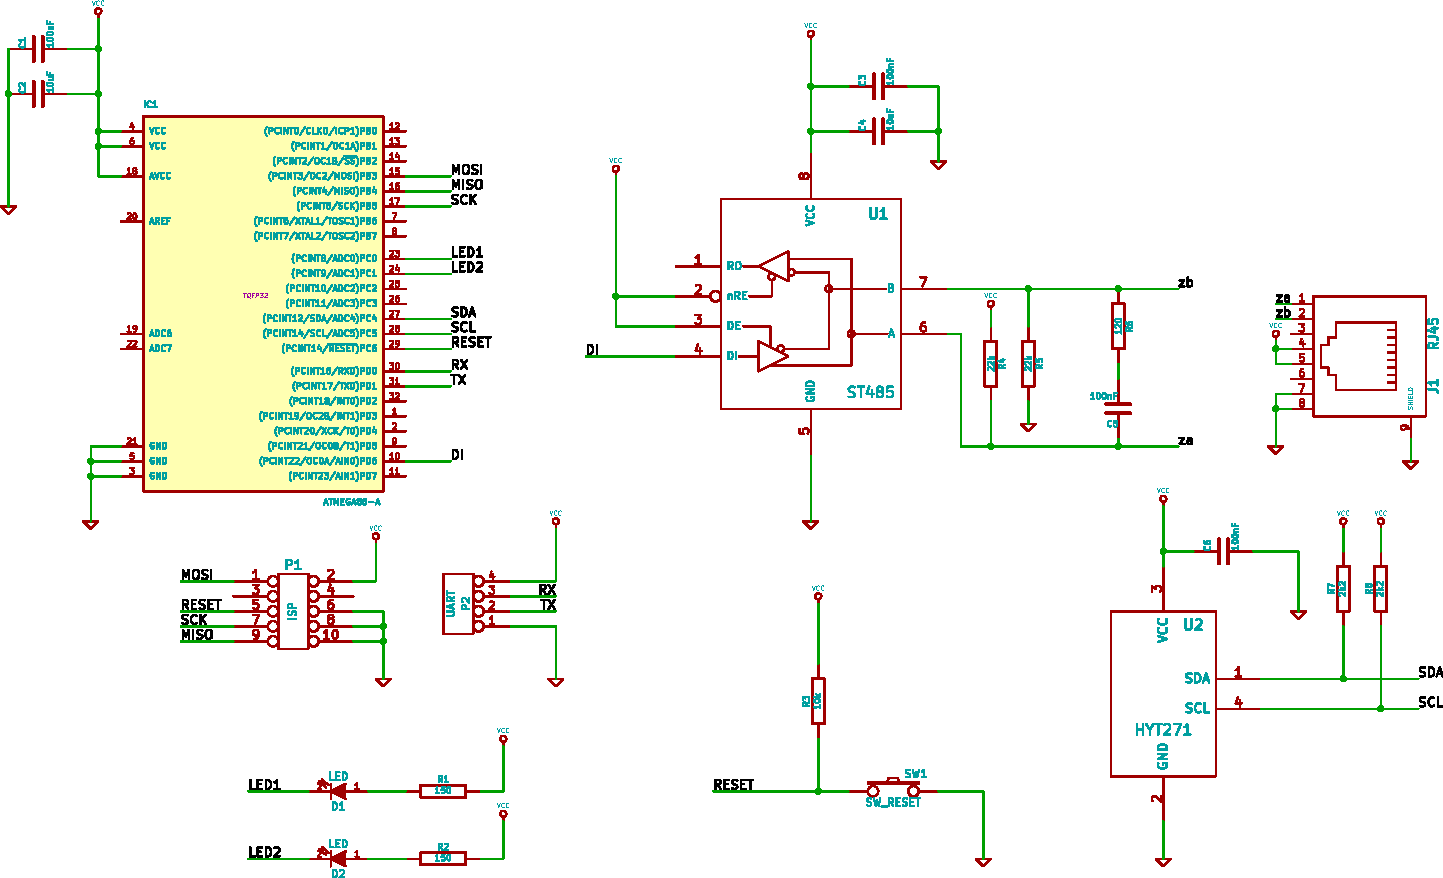
\includegraphics[width=0.8\textwidth]{img/schem_humidity_board.pdf}
	\caption{Humidity board schematic}
	\label{fig:schem_hum}
\end{figure}
\subsection{Software}
\section{Collector board}
The collector board decodes the ZAC protocol and provides an I2C interface for
reading out temperature, as well as humidity values of connected sensors.
Care was taken, to ensure a response time of $<1\,\mathrm{s}$.
\subsection{Hardware}
\begin{figure}
	\centering
	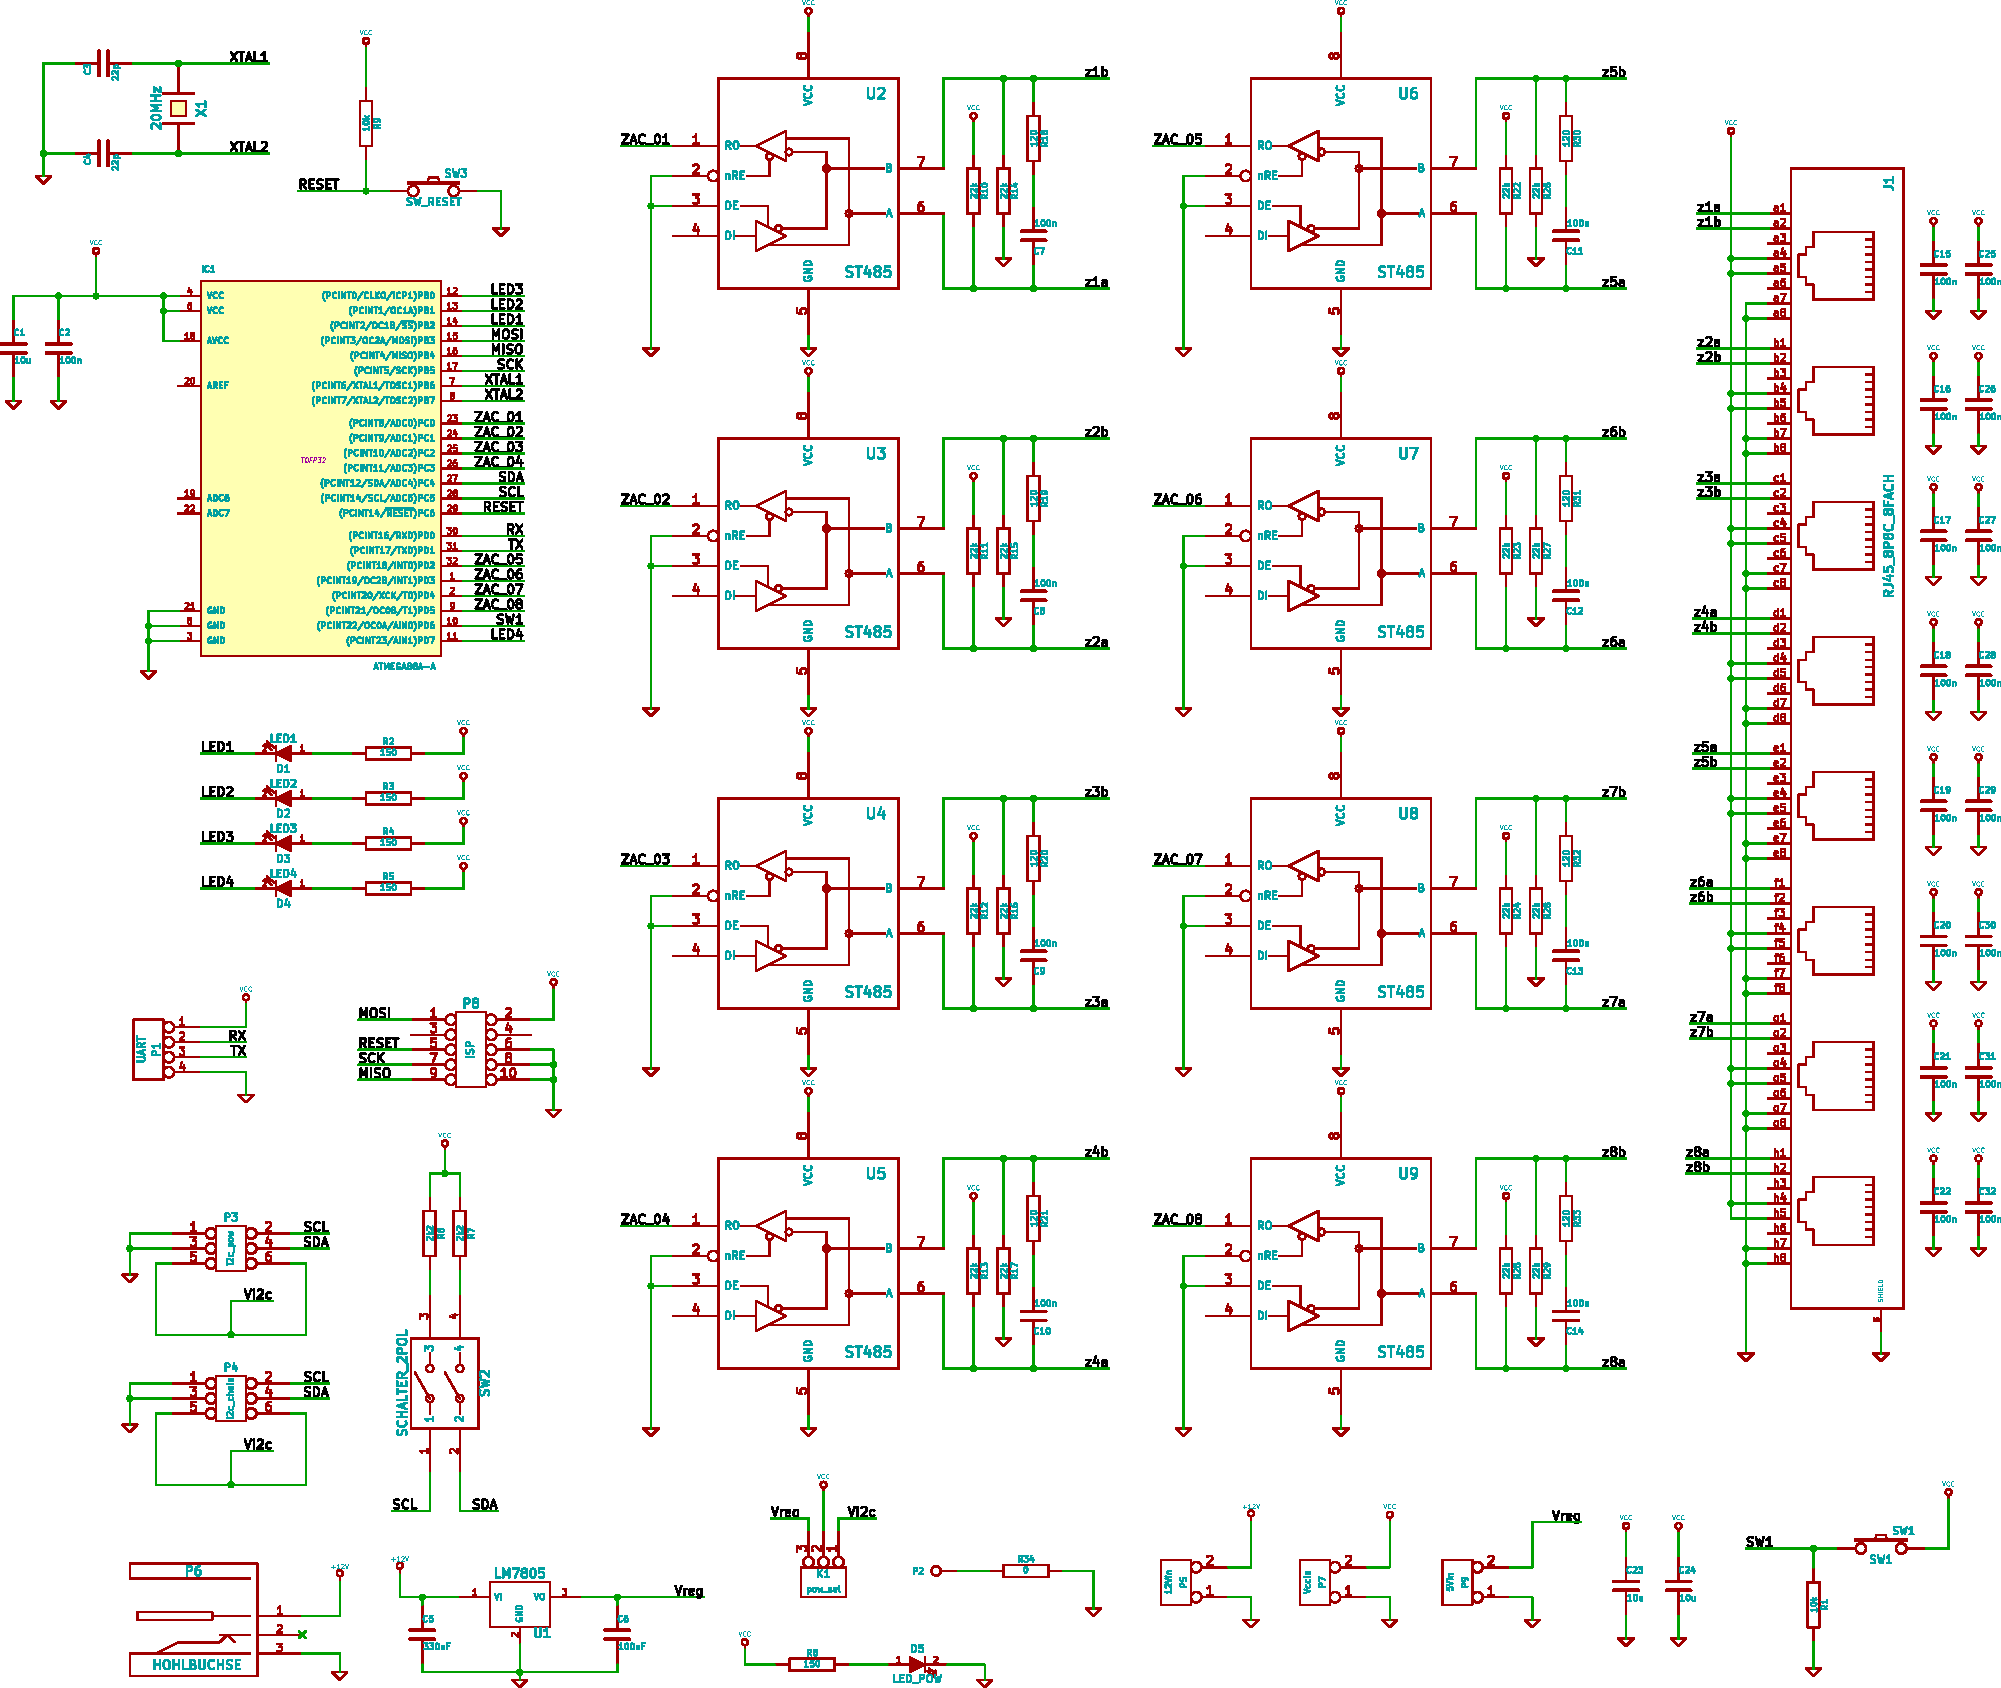
\includegraphics[width=1\textwidth]{img/schem_collector_board.pdf}
	\caption{Collector board schematic}
	\label{fig:schem_collect}
\end{figure}
\subsection{ZAC decoding}
AVR controllers do not have hardware support for decoding the ZAC one wire
protocol (protocol definition is explained in chapter \ref{chap:zac}). Hence we
implemented a software decoder. However our implementation
does not follow the method suggested by \cite{zac} because of timing reasons.\\
To decode one ZAC protocol sensor, we use one 8 bit timer, the corresponding timer
overflow interrupt and the pin change interrupt (PCINT) of the pin, connected to the sensor.
\paragraph{Pin change Interrupt:} On every pin change interrupt, the following actions are executed:\\
Every time:
\begin{itemize}
	\item The current current value is stored to a temporary variable $T_{timer}$, to be able to still access it later.
	\item The timer is reset.
	\item If the timer is not jet running, it is started now.
\end{itemize}
On a falling edge:
\begin{itemize}
	\item If $\left|T_{low} - T_{timer}\right| < T_{thresh}$ with a constant $T_{thresh} << T_{crit}$, we
		have observed a start bit.\\
		We now update the critical sampling time\footnote{$T_{crit} = 0.5\cdot(T_{timer} + T_{low})$ would
		be more accurate, but would consume more time to calculate.}: $T_{crit} = T_{timer}$.
\end{itemize}
On a rising edge:
\begin{itemize}
	\item The current timer value is stored as $T_{low}$. If we already observed a falling edge, this
		represents the time, the signal was low.
	\item If we already have seen a start bit, we now sample a data bit\footnote{Note, that a repeated
		start bit would also be sampled as a data bit with an unpredictable value.}:\\
	$\mathrm{bit} = \begin{cases} 1 & \text{if } T_{timer}<T_{crit} \\ 0 & \text{else}\end{cases}$
\end{itemize}
\paragraph{Timer overflow Interrupt:} The timer is configured in a way, that an overflow will occur after
the timer is running without a reset for $T_{ovf}$, with $T_{bit} < T_{ovf} < 100\,\mathrm{ms}$. Hence
the interrupt will occur, after a completed transmission and before the start of the next transmission.\\
After a overflow occurs, we check, if we received a whole transmission. If this is the case, we disable
interrupts and stop the current measurement. Otherwise we reset the receive buffer and wait for the
next transmission to begin.
\paragraph{Starting a measurement:} To start the meassuring process, the following is executed:
\begin{itemize}
	\item $T_{crit}$ is set to the maximum value.
	\item $T_{low}$ is set to the minimum value. This will ensure, that we do not
		accidentally recognize the first falling edge as a start bit.
	\item The receive buffer is reset.
	\item Interrupts are enabled.
\end{itemize}
\paragraph{}
Our algorithm is not able to see stop bits correctly, if $T_{ovf}$ is configured badly.
However in our case we deliberately configured $T_{ovf}$ to be bigger that the maximum
high time in case of a stop bit.
This allows us to only see the end of the complete transmission, as a TSIC sensor also
sends a useless stop bit after the first 9 bits.
\paragraph{}
As we have up to 8 sensors connected to the Atmega88, we have to do one measurement
after another. as one sample of a measurement takes $>100\,\mathrm{ms}$ we would run
into problems reaching the desired sampling rate of $>1\,\mathrm{Hz}$.
Our approach is to sample two sensors at the
same time, using a second 8 bit timer. Our interrupt handler for the ZAC protocol decoding are not interruptable.
Hence, incomming interrupts are delayed for the runtime $t_e$ of currently executed interrupts.
If we have interrupts active for two sensors at the same time, the controller might see a delayed signal.
\begin{figure}[b]
	\centering
	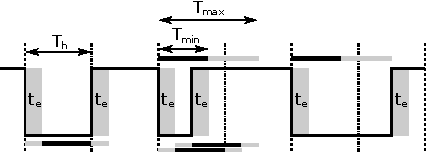
\includegraphics[width=0.7\textwidth]{img/zac_timing.pdf}
	\caption{ZAC protocol worst case timing. The grey shaded areas illustrate the potentially delayed vision
	of a microcontroller due to interrupt latency.}
	\label{fig:zactiming}
\end{figure}
Figure \ref{fig:zactiming} illustrates this problem:\\
When sampling the start bit we get an error for our critical time $T_{crit}$:
$$T_{min} := T_h - t_e < T_{crit} < T_h + t_e$$
When using $T_{crit}$ to determine a bit value, we are again influenced by the possibly delayed preceeding falling edge. We get:
$$T_{min} < T_{crit}' < T_h + 2 \cdot t_e =: T_{max}$$
Our algorithm will only work correctly, if
$$T_{min} > 0.5\cdot T_h + t_e$$
or
$$T_{max} < \frac{3}{2}\cdot T_h\text{.}$$
Both inequations simplify to
$$t_e < \frac{1}{4}\cdot T_h\text{.}$$
According to \cite{zac}, the nominal value for $T_h$ is $\frac{125}{2}\,\mu\mathrm{s}$. Hence our error due to
interrupt latency has to be smaller than $15.625\,\mu\mathrm{s}$.\\
As the microcontroller runs at a clock speed of $20\,\mathrm{MHz}$, we have to complete previous interrupts,
start the interrupt handler of the new interrupt and sample the current timer value within 332 clock cycles,
to not harm the above limit on the error.\\
We implemented a simple branch aware Worst Case Execution Time (WCET) analyzer for the AVR instruction set.
It is able to calculate the maximum execution time of individual sections in the compiled code\footnote{Note that,
whereas branches are considered, only branches to addresses in the future are handled correctly. Loops i.e.
branches to already executed code cause undefined, possibly non terminating behaviour of the analyzer. As our code
does not contain loops, this did not cause problems and loop handling was not implemented.}. Figure \ref{fig:wcet}
shows the WCET analyzer output for the Pin change interrupt handler. The worst case execution time for the total
handler is $100$ cycles. The timer interrupt takes less than $50$ cycles to complete. For a complete analysis one
additionally has to consider the time for jumping to the interrupt handler ($<20$ cycles) and the time we need to read out the
timer value in the new interrupt handler ($<29$ cycles). This gives us a total latency of less than $199$ clock
cycles, which is well within the allowed range.
\begin{figure}
	\centering
	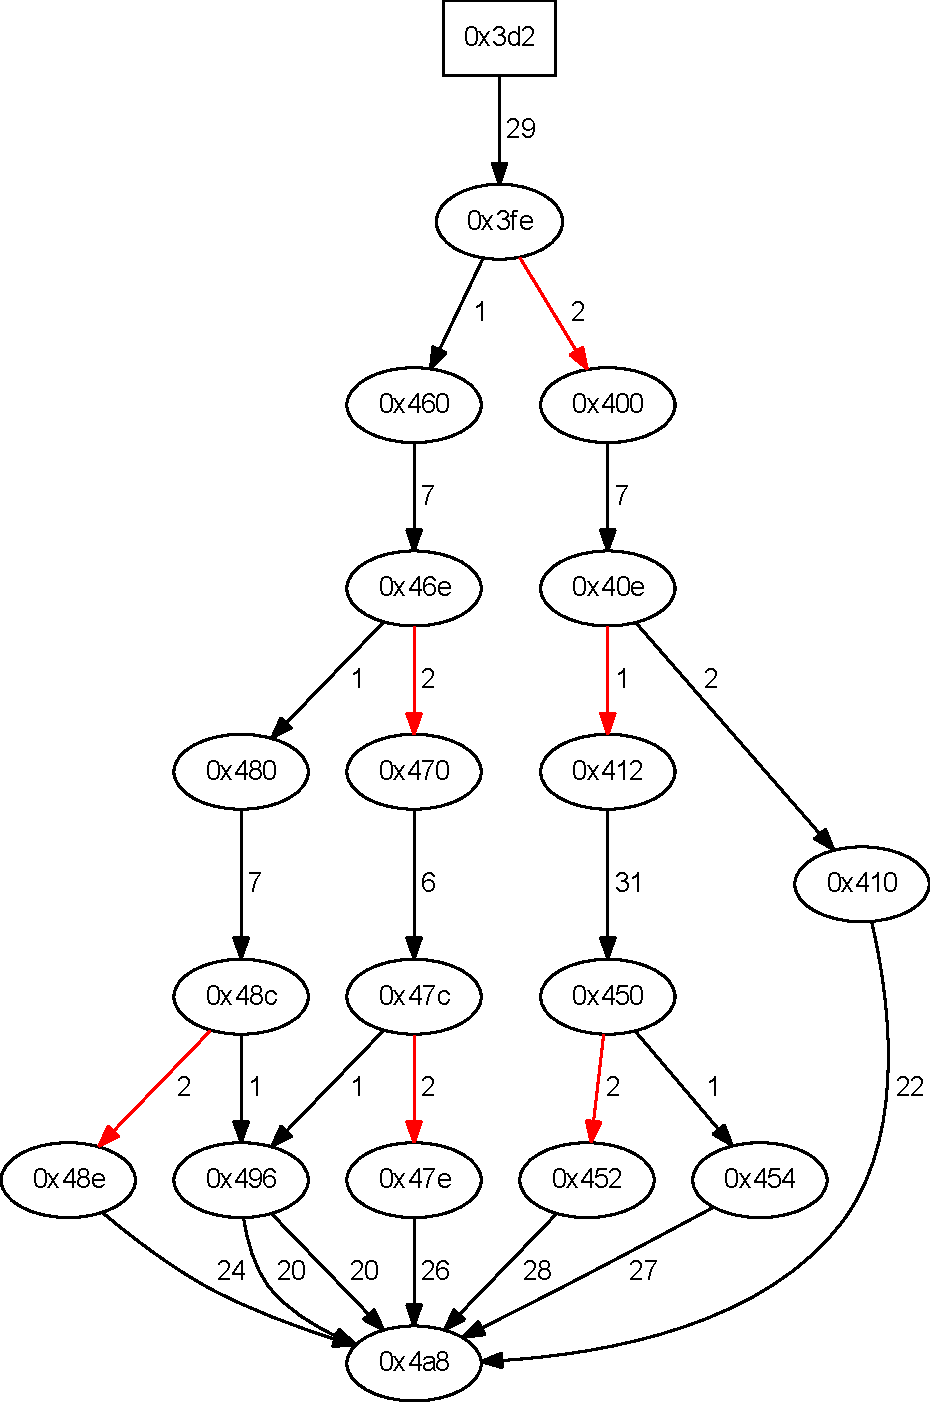
\includegraphics[width=0.5\textwidth]{img/wcet/vector_4.pdf}
  \caption{Branch aware WCET analysis of the Interrupt handler for vector\_4 (Pin change interrupt).
  Nodes represent program addresses, arrows represent branches. Red arrows point to the branch with the
highest execution time. The values near the arrows represent the execution time from the previous node's
address to the instruction causing the branch.}
	\label{fig:wcet}
\end{figure}

\subsection{I2C interface}
Communication with the collector board is done via I2C (Two Wire Interface). Thereby the board acts as an
I2C slave, extending the clock, if it is currently not able to process incomming data.
This is especially used while a measurement is in progress: As soon as new data byte arrives,
it is buffered and the clock will be extended, signalling to the master, that no further data should be sent or received.\\
If a write request (SLA+W) is sent, the following data is interpreted as a command. A list of implemented commands is given
in table \ref{tab:i2c}. The collector board reacts to the general call address 0. This makes it possible to trigger a measurement
on multiple boards, using only one I2C transmission. Also the own I2C address can be set to a new value without knowing the old one.\\
If a read request (SLA+R) is sent, the packet array from the last completed measurement will be sent out, starting with sensor 0.
For details about the packet format see chapter \ref{chap:packet}. Not all packets have to be received, as soon as a STOP bit is
received, the transmission is aborted. A new read request will again trigger the transmission of data starting at sensor 0.
\begin{table}[Hh!]
	\centering
	\begin{tabularx}{\textwidth}{ | c | c | c | X | }
		\hline
    Name & Value & Parameters & Action\\
		\hline
		\hline
    START\_MEASUREMENT & 0x01 & --- & All 8 sensor values will be captured as soon as the STOP bit is received. If during measurement
		the slave is addressed again, the I2C clock will immediately be extended until the measurement is complete, blocking the whole I2C bus.\\
		\hline
    SET\_ADDRESS & 0x02 & address & The own I2C address will be updated with the 1 byte value following the command. The address should
		be in the range from 8 to 112. The default address is 42\\
		\hline
    LED\_ON & 0x03 & number & The LED with the given number will be turned on.\\
		\hline
    LED\_OFF & 0x04 & number & The LED with the given number will be turned off.\\
		\hline
	\end{tabularx}
	\caption{List of implemented I2C commands}
	\label{tab:i2c}
\end{table}
\subsection{Measurement packet format}\label{chap:packet}
After data was received via the ZAC-Wire protocol, it is interpreted and converted to a convenient packet format, suitable for
redirection via I2C. Each packet's integrity is protected by a CRC checksum and consists of the following fields:\\
\begin{description}
	\item[\textbf{type}] This field pecifies the type of the sensor, which supplied the data. Currently implemented values are 0
		for TSIC and 1 for HYT. In case the type field reads 0, the \emph{Humidity} field will have no relevant value hence
		represents a padding field.
	\item[c] This bit is set to 1, if the measurement was completed without a timeout. This is usually the case, when a
		sensor is connected. Hence this bit can be used to determine, whether a sensor is connected or not.
	\item[error] This field reads 1, when an error during sampling has occured. Possible causes are: HYT Checksum missmatch,
		TSIC Parity missmatch or TSIC Protocol format error.
	\item[Temperature] $T_m \cdot 100$ with $T_m$ the measured temperature in Celsius.
	\item[Humidity] $RH_m \cdot 100$ with $RH_m$ the measured relative humidity in \%.
	\item[CRC-8] Checksum over the first 5 bytes of the packet\footnote{The Humidity field is always part of the checksum
		calculation, even if the packet type is 0.}.
\end{description}
Figure \ref{fig:packet} shows the structure of a packet. Packets can be received via I2C in the order, shown in
figure \ref{fig:packetorder}.\\

\begin{figure}
	\centering
	\definecolor{lightgray}{gray}{0.8}
	\begin{bytefield}[endianness=big, bitwidth=2.1em]{8}
		\bitheader{0-7}\\
		\begin{rightwordgroup}{Header}
			\bitbox{2}{type} & \bitbox{3}{\color{lightgray}\rule{\width}{\height}} & \bitbox{1}{c} & \bitbox{2}{error}
		\end{rightwordgroup}\\
		\begin{rightwordgroup}{Payload}
			\wordbox{2}{Temperature}\\
			\wordbox{2}{Humidity}
		\end{rightwordgroup}\\
		\wordbox{1}{CRC-8}
	\end{bytefield}
  \caption{Packet format of a measurement. The whole packet is 6 bytes long}
	\label{fig:packet}
\end{figure}
\begin{figure}
	\centering
	\definecolor{lightgray}{gray}{0.8}
	\begin{bytefield}[endianness=little, bitwidth=0.7em]{48}
		\bitheader{0,6,12,18,24,30,36,42}\\
		\bitbox{6}{Sensor 0} &
		\bitbox{6}{Sensor 1} &
		\bitbox{6}{Sensor 2} &
		\bitbox{6}{Sensor 3} &
		\bitbox{6}{Sensor 4} &
		\bitbox{6}{Sensor 5} &
		\bitbox{6}{Sensor 6} &
		\bitbox{6}{Sensor 7}
	\end{bytefield}
  \caption{Transmission packet order}
	\label{fig:packetorder}
\end{figure}

\section{Ethernet board}
\subsection{Hardware}
\subsection{Software}
\subsection{User interface}
\chapter{References}
%\renewcommand\refname{\vskip -1cm}
%\bibliographystyle{abbrv}
\bibliographystyle{plain}
\begingroup
\def\chapter*#1{}
\bibliography{bib}
\endgroup
%\bibliography{bib}
\nocite{*}

\end{document}
